%%-----------------------------------------------------------------------%%
%%--- Introduction to Graph Theory --------------------------------------%%

\chapter{Introduction to Graph Theory}


%%-----------------------------------------------------------------------%%
%%--- Graphs and digraphs -----------------------------------------------%%

\section{Graphs and digraphs}

\begin{definition}
\textbf{Graphs.}
A \emph{graph} $G = (V, E)$ is an ordered pair of sets. Elements of
$V$ are called \emph{vertices} or \emph{nodes}, and elements of
$E \subseteq V \times V$ are called \emph{edges} or \emph{lines}. We
refer to $V$ as the vertex set of $G$, with $E$ being the edge
set. The cardinality of $V$ is called the \emph{order} of $G$, and
$|E|$ is called the \emph{size} of $G$.
\end{definition}

If $(v_1, v_2) \in E$ is an edge of a graph $G = (V, E)$, we say that
$v_1$ and $v_2$ are \emph{adjacent} vertices. For ease of notation, we
write the edge $(v_1, v_2)$ as $v_1 v_2$. The edge $v_1 v_2$ is also
said to be \emph{incident} with the vertices $v_1$ and $v_2$.

\begin{figure}[!htbp]
\centering
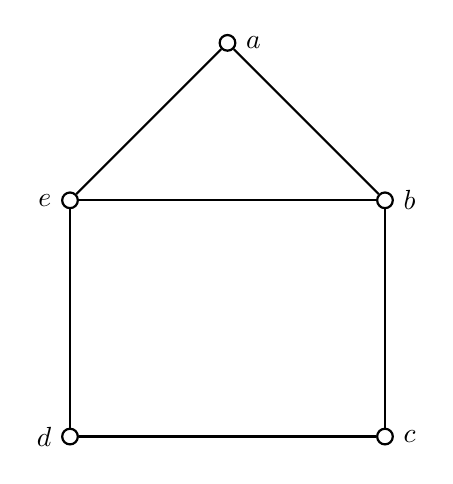
\begin{tikzpicture}
[nodedecorate/.style={shape=circle,inner sep=2pt,draw,thick},%
  linedecorate/.style={-,thick}]
% nodes or vertices
\node (a) at (0,5) [nodedecorate] {};
\node [right] at (a.east) {$a$};
\node (b) at (2,3) [nodedecorate] {};
\node [right] at (b.east) {$b$};
\node (e) at (-2,3) [nodedecorate] {};
\node [left] at (e.west) {$e$};
\node (c) at (2,0) [nodedecorate] {};
\node [right] at (c.east) {$c$};
\node (d) at (-2,0) [nodedecorate] {};
\node [left] at (d.west) {$d$};
% edges or lines
\path
(a) edge[linedecorate] node {} (b)
(b) edge[linedecorate] node {} (c)
(b) edge[linedecorate] node {} (e)
(c) edge[linedecorate] node {} (d)
(d) edge[linedecorate] node {} (e)
(e) edge[linedecorate] node {} (a);
\end{tikzpicture}
\caption{A house graph.}
\label{fig:introduction:house_graph}
\end{figure}

\begin{exercise}
\label{ex:introduction:house_graph}
Consider the graph in Figure~\ref{fig:introduction:house_graph}.
%
\begin{enumerate}
\item List the vertex and edge sets of the graph.

\item For each vertex, list all vertices that are adjacent to it.

\item Which vertex or vertices have the largest number of adjacent
  vertices? Similarly, which vertex or vertices have the smallest
  number of adjacent vertices?

\item If all edges of the graph are removed, is the resulting figure
  still a graph? Why or why not?

\item If all vertices of the graph are removed, is the resulting
  figure still a graph? Why or why not?
\end{enumerate}
\end{exercise}

\begin{proof}[Solution]
(1) Let $G = (V, E)$ denote the graph in
Figure~\ref{fig:introduction:house_graph}. Then the vertex set of $G$
is $V = \{ a, b, c, d, e \}$. The edge set of $G$ is given by
\begin{equation}
\label{eq:introduction:edges_of_house_graph}
E
=
\{ ab, ae, ba, bc, be, cb, cd, dc, de, ed, eb, ea \}.
\end{equation}
We can also use Sage to construct the graph $G$ and list its vertex
and edge sets:
%
\begin{center}
\fontsize{10pt}{10pt}
\selectfont
\tt
\begin{lstlisting}
sage: G = Graph({"a": ["b", "e"], "b": ["a", "c", "e"], "c": ["b", "d"], \
....: "d": ["c", "e"], "e": ["a", "b", "d"]})
sage: G
Graph on 5 vertices
sage: G.vertices()
['a', 'b', 'c', 'd', 'e']
sage: G.edges(labels=False)
[('a', 'b'), ('a', 'e'), ('b', 'e'), ('c', 'b'), ('c', 'd'), ('e', 'd')]
\end{lstlisting}
\end{center}
%
The graph $G$ is undirected, meaning that we do no impose direction on
any edges. Without any direction on the edges, the edge $ab$ is the
same as the edge $ba$. That is why \texttt{G.edges()} returns six
edges instead of the 12 edges listed
in~(\ref{eq:introduction:edges_of_house_graph}).

(2) Let $\text{adj}(v)$ be the set of all vertices that are adjacent
to $v$. Then we have
%
\begin{align*}
\text{adj}(a) &= \{ b, e \} \\
\text{adj}(b) &= \{ a, c, e \} \\
\text{adj}(c) &= \{ b, d \} \\
\text{adj}(d) &= \{ c, e \} \\
\text{adj}(e) &= \{ a, b, d \}
\end{align*}
%
The vertices adjacent to $v$ are also referred to as its
neighbours. We can use the function \texttt{G.neighbors()} to list all
the neighbours of each vertex.
%
\begin{center}
\fontsize{10pt}{10pt}
\selectfont
\tt
\begin{lstlisting}
sage: G.neighbors("a")
['b', 'e']
sage: G.neighbors("b")
['a', 'c', 'e']
sage: G.neighbors("c")
['b', 'd']
sage: G.neighbors("d")
['c', 'e']
sage: G.neighbors("e")
['a', 'b', 'd']
\end{lstlisting}
\end{center}

(3) Taking the cardinalities of the above five sets, we get
$|\text{adj}(a)| = |\text{adj}(c)| = |\text{adj}(d)| = 2$ and
$|\text{adj}(b)| = |\text{adj}(e)| = 3$. Thus $a$, $c$ and $d$ have
the smallest number of adjacent vertices, while $b$ and $e$ have the
largest number of adjacent vertices.

(4) If all the edges in $G$ are removed, the result is still a graph,
although one without any edges. By definition, the edge set of any
graph is a subset of $V \times V$. Removing all edges of $G$ leaves us
with the empty set $\emptyset$, which is a subset of every set.

(5) Say we remove all of the vertices from the graph in
Figure~\ref{fig:introduction:house_graph} and in the process all edges
are removed as well. The result is that both of the vertex and edge
sets are empty. This is a special graph known as an \emph{empty} or
\emph{null} graph.
\end{proof}

In Figure~\ref{fig:introduction:house_graph}, the edges $ae$ and $ea$
represent one and the same edge. If we do not consider the direction
of the edges in the graph of
Figure~\ref{fig:introduction:house_graph}, then the graph has six
edges. However, if the direction of each edge is taken into account,
then there are 12 edges as listed
in~(\ref{eq:introduction:edges_of_house_graph}). The following
definition captures the situation where the direction of the edges are
taken into account.

\begin{definition}
\textbf{Directed graphs.}
A \emph{directed edge} is an edge such that one vertex incident with it
is designated as the head vertex and the other incident vertex is
designated as the tail vertex. A directed edge is said to be directed
from its tail to its head. A \emph{directed graph} or \emph{digraph} is
a graph such that each of whose edges is directed.
\end{definition}

The edges of a digraph can be visually represented as directed arrows,
similarly to the digraph in
Figure~\ref{fig:introduction:directed_triangle_graph}. The graph in
Figure~\ref{fig:introduction:directed_triangle_graph} has the vertex
set $\{ a, b, c \}$ and the edge set $\{ ab, bc, ca \}$. There is an
arrow from vertex $a$ to vertex $b$, hence $ab$ is in the edge
set. However, there is no arrow from $b$ to $a$, so $ba$ is not in the
edge set of the graph in
Figure~\ref{fig:introduction:directed_triangle_graph}.

\begin{figure}[!htbp]
\centering
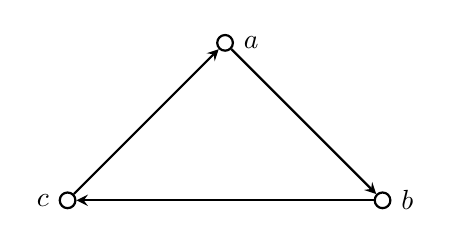
\begin{tikzpicture}
[nodedecorate/.style={shape=circle,inner sep=2pt,draw,thick},%
  arrowdecorate/.style={->,>=stealth,thick}]
% nodes or vertices
\node (c) at (-2,0) [nodedecorate] {};
\node [left] at (c.west) {$c$};
\node (b) at (2,0) [nodedecorate] {};
\node [right] at (b.east) {$b$};
\node (a) at (0,2) [nodedecorate] {};
\node [right] at (a.east) {$a$};
% edges or lines
\path
(a) edge[arrowdecorate] node {} (b)
(b) edge[arrowdecorate] node {} (c)
(c) edge[arrowdecorate] node {} (a);
\end{tikzpicture}
\caption{A triangle as a directed graph.}
\label{fig:introduction:directed_triangle_graph}
\end{figure}

For any vertex $v$ in a graph $G = (V, E)$, the cardinality of
$\text{adj}(v)$ is called the \emph{degree} of $v$ and written as
$\deg(v) = |\text{adj}(v)|$. The degree of $v$ counts the number of
vertices in $G$ that are adjacent to $v$. If $\deg(v) = 0$, we say
that $v$ is an \emph{isolated} vertex. For example, in the graph in
Figure~\ref{fig:introduction:house_graph}, we have $\deg(b) = 3$. For
the graph in Figure~\ref{fig:introduction:directed_triangle_graph}, we
have $\deg(b) = 2$. If $V \neq \emptyset$ and $E = \emptyset$, then
$G$ is a graph consisting entirely of isolated vertices. From
Exercise~\ref{ex:introduction:house_graph} we know that the vertices
$a, c, d$ in Figure~\ref{fig:introduction:house_graph} have the
smallest degree in the graph of that figure, while $b, e$ have the
largest degree. The minimum degree among all vertices in $G$ is
denoted $\delta(G)$, whereas the maximum degree is written as
$\Delta(G)$. Thus, if $G$ denotes the graph in
Figure~\ref{fig:introduction:house_graph} then we have $\delta(G) = 2$
and $\Delta(G) = 3$. In the following Sage session, we construct the
digraph in Figure~\ref{fig:introduction:directed_triangle_graph} and
computes its maximum and minimum number of degrees.
%
\begin{center}
\fontsize{10pt}{10pt}
\selectfont
\tt
\begin{lstlisting}
sage: G = DiGraph({"a": "b", "b": "c", "c": "a"})
sage: G
Digraph on 3 vertices
sage: G.degree("a")
2
sage: G.degree("b")
2
sage: G.degree("c")
2
\end{lstlisting}
\end{center}
%
So for the graph $G$ in
Figure~\ref{fig:introduction:directed_triangle_graph}, we have
$\delta(G) = \Delta(G) = 2$.

The graph $G$ in Figure~\ref{fig:introduction:directed_triangle_graph}
has the special property that its minimum degree is the same as its
maximum degree, i.e. $\delta(G) = \Delta(G)$. Graphs with this
property are referred to as \emph{regular}. An $r$-\emph{regular}
graph is a regular graph each of whose vertices has degree $r$. For
instance, $G$ is a $2$-regular graph. The following result, due to
Euler, counts the total number of degrees in any graph.

\begin{theorem}
\label{thm:introduction:degree_sum}
\textbf{Euler.}
If $G = (V, E)$ is a graph, then $\sum_{v \in V} \deg(v) = 2 |E|$.
\end{theorem}

\begin{proof}
Each edge $e = v_1 v_2 \in E$ is incident with two vertices, so $e$ is
counted twice towards the total sum of degrees. The first time, we count
$e$ towards the degree of the vertex $v_1$, and the second time we
count $e$ towards the degree of $v_2$.
\end{proof}

As $E \subseteq V \times V$, then $E$ can be the empty set, in which
case the total degree of $G = (V, E)$ is zero. Where $E \neq
\emptyset$, then the total degree of $G$ is greater than zero. By
Theorem~\ref{thm:introduction:degree_sum}, the total degree of $G$ is
non-negative and even. This result is an immediate consequence of
Theorem~\ref{thm:introduction:degree_sum} and is captured in the
following corollary.

\begin{corollary}
If $G$ is a graph, then its total number of degrees is non-negative
and even.
\end{corollary}

If $G = (V, E)$ is an $r$-regular graph with $n$ vertices and $m$
edges, it is clear by definition of $r$-regular graphs that the total
degree of $G$ is $rn$. By Theorem~\ref{thm:introduction:degree_sum} we
have $2m = rn$ and therefore $m = rn / 2$. This result is captured in
the following corollary.

\begin{corollary}
If $G = (V, E)$ is an $r$-regular graph having $n$ vertices and $m$
edges, then $m = rn / 2$.
\end{corollary}


%%-----------------------------------------------------------------------%%
%%--- Subgraphs and other graph types -----------------------------------%%

\section{Subgraphs and other graph types}


%%-----------------------------------------------------------------------%%

\subsection{Walks, trails and paths}

If $u$ and $v$ are two vertices in a graph $G$, a $u$-$v$ \emph{walk}
is an alternating sequence of vertices and edges starting with $u$ and
ending at $v$. Consecutive vertices and edges are incident. For the
graph in Figure~\ref{fig:introduction:types_of_walks}, an example of a
walk is an $a$-$e$ walk: $a, b, c, b, e$. In other words, we
start at vertex $a$ and travel to vertex $b$. From $b$, we go to $c$
and then back to $b$ again. Then we end our journey at $e$. Notice
that consecutive vertices in a walk are adjacent to each other. One
can think of vertices as destinations and edges as footpaths, say. We
are allowed to have repeated vertices and edges in a walk. The number
of edges in a walk is called its \emph{length}. For instance, the
walk $a, b, c, b, e$ has length $4$.

\begin{figure}[!htbp]
\centering
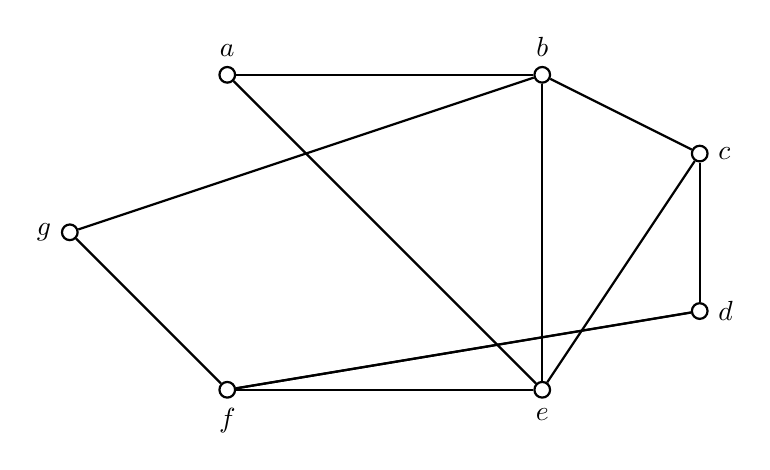
\begin{tikzpicture}
[nodedecorate/.style={shape=circle,inner sep=2pt,draw,thick},%
  linedecorate/.style={-,thick}]
% nodes or vertices
\node (b) at (4,4) [nodedecorate] {};
\node [above] at (b.north) {$b$};
\node (a) at (0,4) [nodedecorate] {};
\node [above] at (a.north) {$a$};
\node (c) at (6,3) [nodedecorate] {};
\node [right] at (c.east) {$c$};
\node (d) at (6,1) [nodedecorate] {};
\node [right] at (d.east) {$d$};
\node (e) at (4,0) [nodedecorate] {};
\node [below] at (e.south) {$e$};
\node (g) at (-2,2) [nodedecorate] {};
\node [left] at (g.west) {$g$};
\node (f) at (0,0) [nodedecorate] {};
\node [below] at (f.south) {$f$};
% edges or lines
\path
(a) edge[linedecorate] node {} (b)
(a) edge[linedecorate] node {} (e)
(b) edge[linedecorate] node {} (c)
(b) edge[linedecorate] node {} (e)
(b) edge[linedecorate] node {} (g)
(c) edge[linedecorate] node {} (d)
(c) edge[linedecorate] node {} (e)
(d) edge[linedecorate] node {} (f)
(d) edge[linedecorate] node {} (f)
(e) edge[linedecorate] node {} (f)
(f) edge[linedecorate] node {} (g);
\end{tikzpicture}
\caption{Walking along a graph.}
\label{fig:introduction:types_of_walks}
\end{figure}

A \emph{trail} is a walk with no repeating edges. For example, the
$a$-$b$ walk $a, b, c, d, f, g, b$ in
Figure~\ref{fig:introduction:types_of_walks} is a trail. It does not
contain any repeated edges, but it contains one repeated vertex,
i.e. $b$. Nothing in the definition of a trail restricts a trail from
having repeated vertices. Where the start and end vertices of a trail
are the same, we say that the trail is a \emph{circuit}, otherwise
known as a \emph{closed} trail. Thus the walk $a, b, e, a$ is a
circuit.

A walk with no repeating vertices is called a \emph{path}. Without any
repeating vertices, a path cannot have repeating edges, hence a path
is also a trail. A path whose start and end vertices are the same is
called a \emph{cycle}. For example, the walk $a, b, c, e, a$
in Figure~\ref{fig:introduction:types_of_walks} is a path and a cycle.

\begin{exercise}
Consider the graph in Figure~\ref{fig:introduction:types_of_walks}.
%
\begin{enumerate}
\item Find two distinct walks that are not trails and determine their
  lengths.

\item Find two distinct trails that are not paths and determine their
  lengths.

\item Find two distinct paths and determine their lengths.

\item Find a circuit that is not a cycle.
\end{enumerate}
\end{exercise}

\begin{proof}[Solution]
(1) Here are two distinct walks that are not trails:
$w_1: g, b, e, a, b, e$ and $w_2: f, d, c, e, f, d$. The length of
walk $w_1$ is 5 and the length of walk $w_2$ is also 5.

(2) Here are two distinct trails that are not paths:
$t_1: a, b, c, d, f$ and $t_2: b, e, f, d, c$. The length of trail
$t_1$ is 4 and the length of trail $t_2$ is also 4.

(3) Here are two distinct paths: $p_1: a, b, c, d, f, e$ and
$p_2: g, b, a, e, f, d$. The length of path $p_1$ is 5 and the length
of path $p_2$ is also 5.

(4) Here is a circuit that is not a cycle: $d, c, e, b, a, e, f, d$.
\end{proof}

A graph is said to be \emph{connected} if for every pair of distinct
vertices $u, v$ there is a $u$-$v$ path joining them. A graph that is
not connected is referred to as \emph{disconnected}. The empty graph
is disconnected and so is any non-empty graph with an isolated
vertex. However, the graph in
Figure~\ref{fig:introduction:directed_triangle_graph} is
connected. A \emph{geodesic path} or \emph{shortest path} between two
distinct vertices $u,v$ of a graph is a $u$-$v$ path of minimum
length. A non-empty graph may have several shortest paths between some
distinct pair of vertices. For the graph in
Figure~\ref{fig:introduction:types_of_walks}, both $a,b,c$ and $a,e,c$
are geodesic paths between $a$ and $c$.

\begin{exercise}
Determine whether or not the graph in
Figure~\ref{fig:introduction:types_of_walks} is connected. Find a
shortest path from $g$ to $d$.
\end{exercise}

\begin{proof}[Solution]
In the following Sage session, we first construct the graph in
Figure~\ref{fig:introduction:types_of_walks} and use the method
\verb!is_connected()! to determine whether or not the graph is
connected. Finally, we use the method \verb!shortest_path()! to find
a geodesic path between $g$ and $d$.
%
\begin{center}
\fontsize{10pt}{10pt}
\selectfont
\tt
\begin{lstlisting}
sage: g = Graph({"a": ["b", "e"], "b": ["a", "g", "e", "c"], \
....: "c": ["b", "e", "d"], "d": ["c", "f"], "e": ["f", "a", "b", "c"], \
....: "f": ["g", "d", "e"], "g": ["b", "f"]})
sage: g.is_connected()
True
sage: g.shortest_path("g", "d")
['g', 'f', 'd']
\end{lstlisting}
\end{center}
\end{proof}


%%-----------------------------------------------------------------------%%

\subsection{Subgraphs, complete and bipartite graphs}

Let $G$ be a graph with vertex set $V(G)$ and edge set
$E(G)$. Consider a graph $H$ such that $V(H) \subseteq V(G)$ and $E(H)
\subseteq E(G)$. Furthermore, if $uv \in E(H)$ then $u,v \in
V(H)$. Then $H$ is called a \emph{subgraph} of $G$ and $G$ is referred
to as a \emph{supergraph} of $H$. Starting from $G$, one can obtain
its subgraph $H$ by deleting edges and/or vertices from $G$. Note that
when a vertex $v$ is removed from $G$, then all edges incident with
$v$ are also removed. If $V(H) = V(G)$, then $H$ is called a
\emph{spanning} subgraph of $G$. In
Figure~\ref{fig:introduction:star_subgraph}, let $G$ be the left-hand
side graph and let $H$ be the right-hand side graph. Then it is clear
that $H$ is a spanning subgraph of $G$. To obtain a spanning subgraph
from a given graph, we delete edges from the given graph.

\begin{figure}[!htbp]
\centering
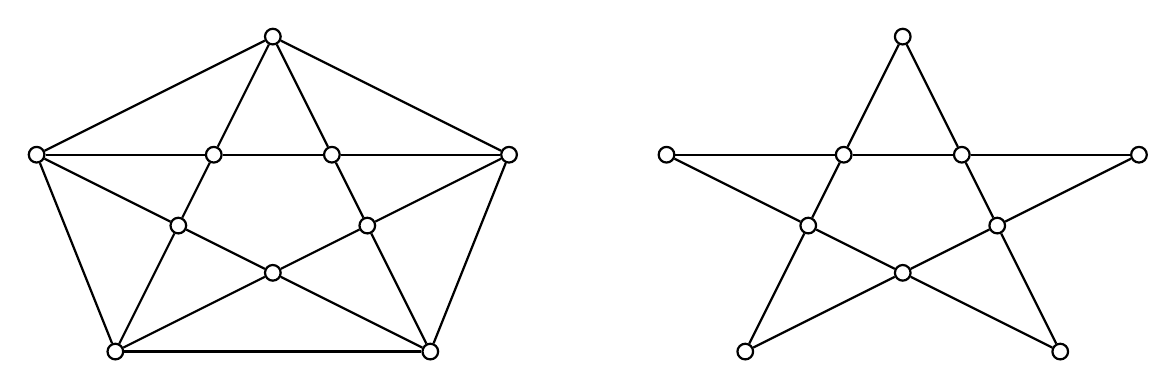
\begin{tikzpicture}
[nodedecorate/.style={shape=circle,inner sep=2pt,draw,thick},%
  linedecorate/.style={-,thick}]
%%% pentagon with star and inner pentagon
% nodes or vertices
\node (a) at (-2,0) [nodedecorate] {};
\node (b) at (2,0) [nodedecorate] {};
\node (c) at (-3,2.5) [nodedecorate] {};
\node (d) at (3,2.5) [nodedecorate] {};
\node (e) at (0,4) [nodedecorate] {};
\node (f) at (-0.75,2.5) [nodedecorate] {};
\node (g) at (-1.2,1.6) [nodedecorate] {};
\node (h) at (0,1) [nodedecorate] {};
\node (i) at (1.2,1.6) [nodedecorate] {};
\node (j) at (0.75,2.5) [nodedecorate] {};
% edges or lines
\path
(a) edge[linedecorate] node {} (b)
(a) edge[linedecorate] node {} (c)
(a) edge[linedecorate] node {} (g)
(a) edge[linedecorate] node {} (h)
(b) edge[linedecorate] node {} (d)
(b) edge[linedecorate] node {} (h)
(b) edge[linedecorate] node {} (i)
(c) edge[linedecorate] node {} (e)
(c) edge[linedecorate] node {} (f)
(c) edge[linedecorate] node {} (g)
(d) edge[linedecorate] node {} (e)
(d) edge[linedecorate] node {} (i)
(d) edge[linedecorate] node {} (j)
(e) edge[linedecorate] node {} (f)
(e) edge[linedecorate] node {} (j)
(f) edge[linedecorate] node {} (g)
(f) edge[linedecorate] node {} (j)
(g) edge[linedecorate] node {} (h)
(h) edge[linedecorate] node {} (i)
(i) edge[linedecorate] node {} (j);
%
%%% star and inner pentagon
% nodes or vertices
\node (a2) at (6,0) [nodedecorate] {};
\node (b2) at (10,0) [nodedecorate] {};
\node (c2) at (5,2.5) [nodedecorate] {};
\node (d2) at (11,2.5) [nodedecorate] {};
\node (e2) at (8,4) [nodedecorate] {};
\node (f2) at (7.25,2.5) [nodedecorate] {};
\node (g2) at (6.8,1.6) [nodedecorate] {};
\node (h2) at (8,1) [nodedecorate] {};
\node (i2) at (9.2,1.6) [nodedecorate] {};
\node (j2) at (8.75,2.5) [nodedecorate] {};
% edges or lines
\path
(a2) edge[linedecorate] node {} (g2)
(a2) edge[linedecorate] node {} (h2)
(b2) edge[linedecorate] node {} (h2)
(b2) edge[linedecorate] node {} (i2)
(c2) edge[linedecorate] node {} (f2)
(c2) edge[linedecorate] node {} (g2)
(d2) edge[linedecorate] node {} (i2)
(d2) edge[linedecorate] node {} (j2)
(e2) edge[linedecorate] node {} (f2)
(e2) edge[linedecorate] node {} (j2)
(f2) edge[linedecorate] node {} (g2)
(f2) edge[linedecorate] node {} (j2)
(g2) edge[linedecorate] node {} (h2)
(h2) edge[linedecorate] node {} (i2)
(i2) edge[linedecorate] node {} (j2);
\end{tikzpicture}
\caption{A graph and one of its subgraphs.}
\label{fig:introduction:star_subgraph}
\end{figure}

We now consider several standard classes of graphs. The \emph{complete}
graph $K_n$ on $n$ vertices is a graph such that any two distinct
vertices are adjacent. As $|V(K_n)| = n$, then $|E(K_n)|$ is
equivalent to the total number of 2-combinations from a set of $n$
objects:
\[
|E(K_n)|
=
\binom{n}{2}
=
\frac{n(n-1)}{2}
\]
Thus for any graph $G$ with $n$ vertices, its total number of edges
$|E(G)|$ is bounded above by
\[
|E(G)|
\leq
\frac{n(n - 1)}{2}
\]
Figure~\ref{fig:introduction:five_complete_graphs} shows complete
graphs each of whose total number of vertices is bounded by
$1 \leq n \leq 5$. The complete graph $K_1$ has one vertex with
no edges. It is also called the \emph{trivial} graph.

\begin{figure}[!htbp]
\centering
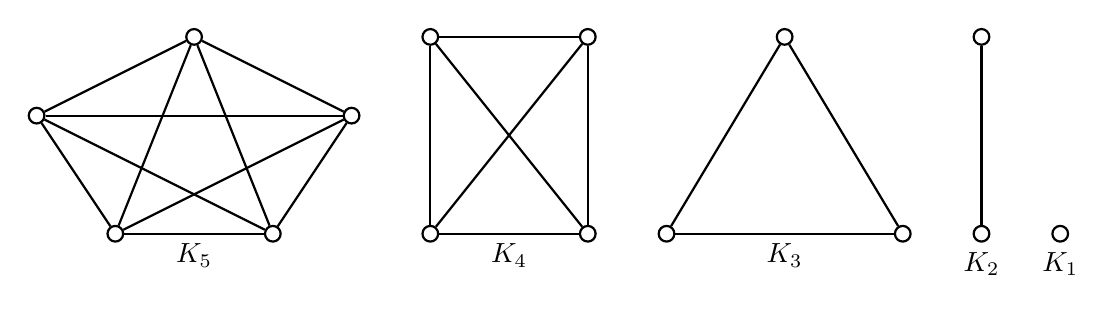
\begin{tikzpicture}
[nodedecorate/.style={shape=circle,inner sep=2pt,draw,thick},%
  linedecorate/.style={-,thick}]
%%% complete graph K_5
% nodes or vertices
\node (a) at (-1,0) [nodedecorate] {};
\node (b) at (1,0) [nodedecorate] {};
\node (c) at (-2,1.5) [nodedecorate] {};
\node (d) at (2,1.5) [nodedecorate] {};
\node (e) at (0,2.5) [nodedecorate] {};
% edges or lines
\path
(a) edge[linedecorate] node[below] {$K_5$} (b)
(a) edge[linedecorate] node {} (c)
(a) edge[linedecorate] node {} (d)
(a) edge[linedecorate] node {} (e)
(b) edge[linedecorate] node {} (c)
(b) edge[linedecorate] node {} (d)
(b) edge[linedecorate] node {} (e)
(c) edge[linedecorate] node {} (d)
(c) edge[linedecorate] node {} (e)
(d) edge[linedecorate] node {} (e);
%
%%% complete graph K_4
% nodes or vertices
\node (a) at (3,0) [nodedecorate] {};
\node (b) at (5,0) [nodedecorate] {};
\node (c) at (3,2.5) [nodedecorate] {};
\node (d) at (5,2.5) [nodedecorate] {};
% edges or lines
\path
(a) edge[linedecorate] node[below] {$K_4$} (b)
(a) edge[linedecorate] node {} (c)
(a) edge[linedecorate] node {} (d)
(b) edge[linedecorate] node {} (c)
(b) edge[linedecorate] node {} (d)
(c) edge[linedecorate] node {} (d);
%
%%% complete graph K_3
% nodes or vertices
\node (a) at (6,0) [nodedecorate] {};
\node (b) at (9,0) [nodedecorate] {};
\node (c) at (7.5,2.5) [nodedecorate] {};
% edges or lines
\path
(a) edge[linedecorate] node[below] {$K_3$} (b)
(a) edge[linedecorate] node {} (c)
(b) edge[linedecorate] node {} (c);
%
%%% complete graph K_2
% nodes or vertices
\node (a) at (10,0) [nodedecorate] {};
\node [below] at (a.south) {$K_2$};
\node (b) at (10,2.5) [nodedecorate] {};
% edges or lines
\path
(a) edge[linedecorate] node {} (b);
%
%%% complete graph K_1
% nodes or vertices
\node (a) at (11,0) [nodedecorate] {};
\node [below] at (a.south) {$K_1$};
\end{tikzpicture}
\caption{Complete graphs $K_n$ for $1 \leq n \leq 5$.}
\label{fig:introduction:five_complete_graphs}
\end{figure}

The \emph{cycle} graph on $n \geq 3$ vertices, denoted $C_n$, is the
connected $2$-regular graph on $n$ vertices. Each vertex in $C_n$ has
degree exactly $2$ and $C_n$ is
connected. Figure~\ref{fig:introduction:four_cycle_graphs} shows
cycles graphs $C_n$ where $3 \leq n \leq 6$. The \emph{path} on
$n \geq 1$ vertices is denoted $P_n$. For $n = 1, 2$ we have
$P_1 = K_1$ and $P_2 = K_2$. Where $n \geq 3$, then $P_n$ is a
spanning subgraph of $C_n$ obtained by deleting one edge.

\begin{figure}[!htbp]
\centering
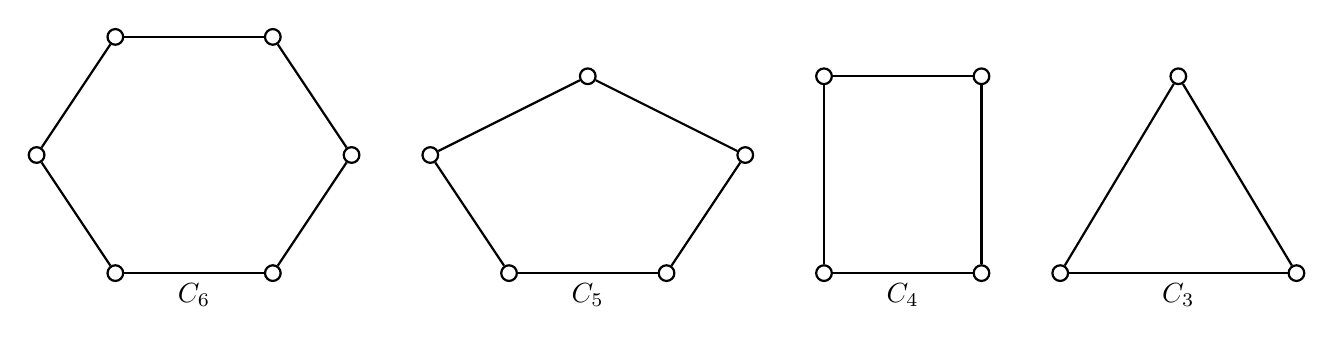
\begin{tikzpicture}
[nodedecorate/.style={shape=circle,inner sep=2pt,draw,thick},%
  linedecorate/.style={-,thick}]
%%% cycle graph C_6
% nodes or vertices
\node (a) at (-6,0) [nodedecorate] {};
\node (b) at (-4,0) [nodedecorate] {};
\node (c) at (-7,1.5) [nodedecorate] {};
\node (d) at (-3,1.5) [nodedecorate] {};
\node (e) at (-6,3) [nodedecorate] {};
\node (f) at (-4,3) [nodedecorate] {};
% edges or lines
\path
(a) edge[linedecorate] node[below] {$C_6$} (b)
(a) edge[linedecorate] node {} (c)
(b) edge[linedecorate] node {} (d)
(c) edge[linedecorate] node {} (e)
(d) edge[linedecorate] node {} (f)
(e) edge[linedecorate] node {} (f);
%
%%% cycle graph C_5
% nodes or vertices
\node (a) at (-1,0) [nodedecorate] {};
\node (b) at (1,0) [nodedecorate] {};
\node (c) at (-2,1.5) [nodedecorate] {};
\node (d) at (2,1.5) [nodedecorate] {};
\node (e) at (0,2.5) [nodedecorate] {};
% edges or lines
\path
(a) edge[linedecorate] node[below] {$C_5$} (b)
(a) edge[linedecorate] node {} (c)
(b) edge[linedecorate] node {} (d)
(c) edge[linedecorate] node {} (e)
(d) edge[linedecorate] node {} (e);
%
%%% cycle graph C_4
% nodes or vertices
\node (a) at (3,0) [nodedecorate] {};
\node (b) at (5,0) [nodedecorate] {};
\node (c) at (3,2.5) [nodedecorate] {};
\node (d) at (5,2.5) [nodedecorate] {};
% edges or lines
\path
(a) edge[linedecorate] node[below] {$C_4$} (b)
(a) edge[linedecorate] node {} (c)
(b) edge[linedecorate] node {} (d)
(c) edge[linedecorate] node {} (d);
%
%%% cycle graph C_3
% nodes or vertices
\node (a) at (6,0) [nodedecorate] {};
\node (b) at (9,0) [nodedecorate] {};
\node (c) at (7.5,2.5) [nodedecorate] {};
% edges or lines
\path
(a) edge[linedecorate] node[below] {$C_3$} (b)
(a) edge[linedecorate] node {} (c)
(b) edge[linedecorate] node {} (c);
\end{tikzpicture}
\caption{Cycle graphs $C_n$ for $3 \leq n \leq 6$.}
\label{fig:introduction:four_cycle_graphs}
\end{figure}

A \emph{bipartite} graph $G$ is a graph with at least two
vertices such that $V(G)$ can be split into two disjoint subsets $V_1$
and $V_2$, both non-empty. Every edge $uv \in E(G)$ is such that
$u \in V_1$ and $v \in V_2$, or $v \in V_1$ and $u \in V_2$. The
\emph{complete bipartite} graph $K_{m,n}$ is the bipartite graph whose
vertex set is partitioned into two non-empty disjoint sets $V_1$ and
$V_2$ with $|V_1| = m$ and $|V_2| = n$. Any vertex in $V_1$ is
adjacent to each vertex in $V_2$, and any two distinct vertices in
$V_i$ are not adjacent to each other. If $m = n$, then $K_{n,n}$ is
$n$-regular. Where $m = 1$ then $K_{1,n}$ is called the \emph{star}
graph. Figure~\ref{fig:introduction:bipartite_complete_bipartite_graphs}
shows a bipartite graph together with the complete bipartite graphs
$K_{4,3}$ and $K_{3,3}$, and the star graph $K_{1,4}$.

\begin{figure}[!htbp]
\centering
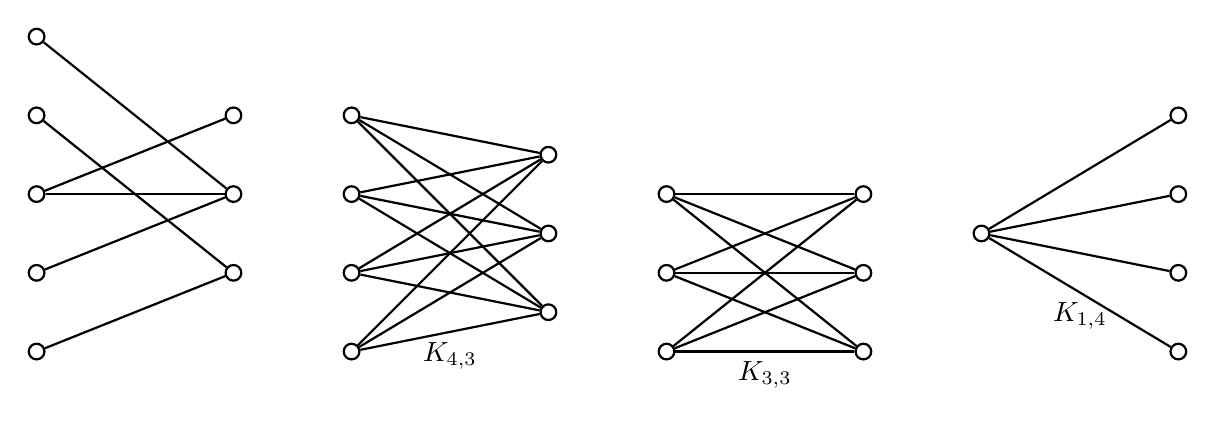
\begin{tikzpicture}
[nodedecorate/.style={shape=circle,inner sep=2pt,draw,thick},%
  linedecorate/.style={-,thick}]
%%% bipartite graph
% nodes or vertices
\node (a) at (0,0) [nodedecorate] {};
\node (b) at (0,1) [nodedecorate] {};
\node (c) at (0,2) [nodedecorate] {};
\node (d) at (0,3) [nodedecorate] {};
\node (e) at (0,4) [nodedecorate] {};
\node (f) at (2.5,3) [nodedecorate] {};
\node (g) at (2.5,2) [nodedecorate] {};
\node (h) at (2.5,1) [nodedecorate] {};
% edges or lines
\path
(a) edge[linedecorate] node {} (h)
(b) edge[linedecorate] node {} (g)
(c) edge[linedecorate] node {} (g)
(c) edge[linedecorate] node {} (f)
(d) edge[linedecorate] node {} (h)
(e) edge[linedecorate] node {} (g);
%
%%% complete bipartite graph K_{4,3}
% nodes or vertices
\node (a) at (4,0) [nodedecorate] {};
\node (b) at (4,1) [nodedecorate] {};
\node (c) at (4,2) [nodedecorate] {};
\node (d) at (4,3) [nodedecorate] {};
\node (e) at (6.5,2.5) [nodedecorate] {};
\node (f) at (6.5,1.5) [nodedecorate] {};
\node (g) at (6.5,0.5) [nodedecorate] {};
% edges or lines
\path
(a) edge[linedecorate] node {} (e)
(a) edge[linedecorate] node {} (f)
(a) edge[linedecorate] node[below] {$K_{4,3}$} (g)
(b) edge[linedecorate] node {} (e)
(b) edge[linedecorate] node {} (f)
(b) edge[linedecorate] node {} (g)
(c) edge[linedecorate] node {} (e)
(c) edge[linedecorate] node {} (f)
(c) edge[linedecorate] node {} (g)
(d) edge[linedecorate] node {} (e)
(d) edge[linedecorate] node {} (f)
(d) edge[linedecorate] node {} (g);
%
%%% complete bipartite graph K_{3,3}
% nodes or vertices
\node (a) at (8,0) [nodedecorate] {};
\node (b) at (8,1) [nodedecorate] {};
\node (c) at (8,2) [nodedecorate] {};
\node (d) at (10.5,2) [nodedecorate] {};
\node (e) at (10.5,1) [nodedecorate] {};
\node (f) at (10.5,0) [nodedecorate] {};
% edges or lines
\path
(a) edge[linedecorate] node {} (d)
(a) edge[linedecorate] node {} (e)
(a) edge[linedecorate] node[below] {$K_{3,3}$} (f)
(b) edge[linedecorate] node {} (d)
(b) edge[linedecorate] node {} (e)
(b) edge[linedecorate] node {} (f)
(c) edge[linedecorate] node {} (d)
(c) edge[linedecorate] node {} (e)
(c) edge[linedecorate] node {} (f);
%
%%% star graph K_{1,4}
% nodes or vertices
\node (a) at (12,1.5) [nodedecorate] {};
\node (b) at (14.5,3) [nodedecorate] {};
\node (c) at (14.5,2) [nodedecorate] {};
\node (d) at (14.5,1) [nodedecorate] {};
\node (e) at (14.5,0) [nodedecorate] {};
% edges or lines
\path
(a) edge[linedecorate] node {} (b)
(a) edge[linedecorate] node {} (c)
(a) edge[linedecorate] node {} (d)
(a) edge[linedecorate] node[below] {$K_{1,4}$} (e);
\end{tikzpicture}
\caption{Bipartite, complete bipartite and star graphs.}
\label{fig:introduction:bipartite_complete_bipartite_graphs}
\end{figure}


%%-----------------------------------------------------------------------%%
%%--- Isomorphic graphs -------------------------------------------------%%

\section{Isomorphic graphs}


%%-----------------------------------------------------------------------%%
%%--- Graph operations --------------------------------------------------%%

\section{Graph operations}


%%-----------------------------------------------------------------------%%
%%--- Graph searching ---------------------------------------------------%%

\section{Graph searching}

\begin{itemize}
\item algorithms for breadth-first and depth-first searchs. Explain
  how these relate to determining a graph's connectivity.

\item algorithms for shortest paths.
\end{itemize}
